\appendix
\chapter{Penelusuran Klaim ke Bukti}

\section{Ketentuan implementasi lintas problem}

\begin{table}[!htbp]
\centering\small
\begin{tabularx}{\textwidth}{@{}L{4.6cm}L{3.8cm}Y@{}}
\toprule
\textbf{Ketentuan di soal} & \textbf{Cara memeriksa} & \textbf{Kode atau bukti}\\
\midrule
Komunikasi lewat jaringan; tidak berbagi library business-logic & \code{pkg/obs} hanya utilitas teknis; tiap service punya \code{go.mod} sendiri & \code{pkg/obs}, \code{services/*/go.mod}\\
Satu storage satu pemilik; Canonical Store hanya diakses Aggregator & \cmd{make demo-isolation} & \code{docs/evidence/p4/isolation.log}\\
Satu container per service; satu perintah orkestrasi & \cmd{make reset} atau \cmd{docker compose up --build} & \code{services/*/Dockerfile}, \code{docker-compose.yml}\\
Kredensial lembaga tidak berlaku lintas instansi & \cmd{make demo-mock-auth} & \code{docs/evidence/p3/mock-auth.log}\\
Tidak ada kredensial di kode atau commit; \code{.env.example} tersedia & \cmd{make secrets} & \code{.env.example}, \code{.gitignore}, \code{.gitleaks.toml}\\
\code{/health}, log terstruktur ber-\code{cid}, latensi panggilan keluar & Langkah 8 demo Problem~1; \code{cid-trace.log} Problem~2 & \code{pkg/obs}\\
Polling dari BNPB, interval dapat diatur, sedikitnya satu event per 10~detik, seed 20 record & Tes mock; demo Problem~1 & \code{services/*-mock/internal/*/generator.go}\\
Kegagalan benar-benar dipicu saat demo & \cmd{make demo-p2-aggregator}, \cmd{make demo-p2} & \cmd{POST /admin/outage}, \cmd{POST /admin/delay}\\
\bottomrule
\end{tabularx}
\caption{Ketentuan implementasi dan cara memeriksanya.}
\end{table}

\section{Matriks kriteria, perintah, dan bukti}

{\small
\begin{longtable}{@{}L{3.3cm}L{4.2cm}L{5.7cm}L{1.5cm}@{}}
\toprule
\textbf{Problem} & \textbf{Perintah} & \textbf{Berkas bukti} & \textbf{Status}\\
\midrule
\endhead
P1 & \cmd{make demo-p1} & \code{docs/evidence/p1/latest.log} & \lulus\\
P2 (ingest) & \cmd{make demo-p2-aggregator} & \code{docs/evidence/p2/aggregator-latest.log} & \lulus\\
P2 (layanan, load test) & \cmd{make demo-p2} & \code{docs/evidence/p2/latest.log}, \code{k6-summary.json}, \code{k6-overload-summary.json}, \code{cid-trace.log} & \lulus\\
P3 (kredensial mock) & \cmd{make demo-mock-auth} & \code{docs/evidence/p3/mock-auth.log} & \lulus\\
P3 (klien downstream) & \cmd{make demo-p3} & \code{docs/evidence/p3/latest.log} & \lulus\\
P3 (tanpa kredensial ter-commit) & \cmd{make secrets} & keluaran \code{scripts/check-secrets.sh} & \lulus\\
P4 (isolasi storage) & \cmd{make demo-isolation} & \code{docs/evidence/p4/isolation.log} & \lulus\\
P4 (JSONB, record berdampingan) & \cmd{make demo-p4} (langkah B--D) & \code{docs/evidence/p4/latest.log} & \lulus\\
P4 (hentikan, bangun ulang, jalankan ulang) & \cmd{make demo-p4} (langkah A) & \code{docs/evidence/p4/latest.log} & \lulus\\
P5 (fan-out, consumer mati, menyusul) & \cmd{make demo-p5} & \code{docs/evidence/p5/latest.log} & \lulus\\
P5 (consumer baru tanpa mengubah producer) & \cmd{make demo-p5} (langkah E) & \code{docs/evidence/p5/latest.log} & \lulus\\
\bottomrule
\end{longtable}
}

\section{Perintah pemeriksaan penuh}

\begin{lstlisting}
make lint && make test-race                                      # kualitas kode dan tes (dengan race detector)
make reset && make demo-p1 demo-p2-aggregator demo-mock-auth demo-isolation
make demo-p4 demo-p5                                             # rebuild satu service, field baru tanpa migrasi, consumer baru
make demo-p2 demo-p3                                             # termasuk load test dan menunggu token kedaluwarsa
make secrets                                                     # sebelum tag milestone-1
\end{lstlisting}

\chapter{Lampiran Surat Pernyataan Penggunaan AI}

Surat pernyataan penggunaan AI yang sudah diisi dan ditandatangani ketiga anggota terlampir pada dua halaman berikut.

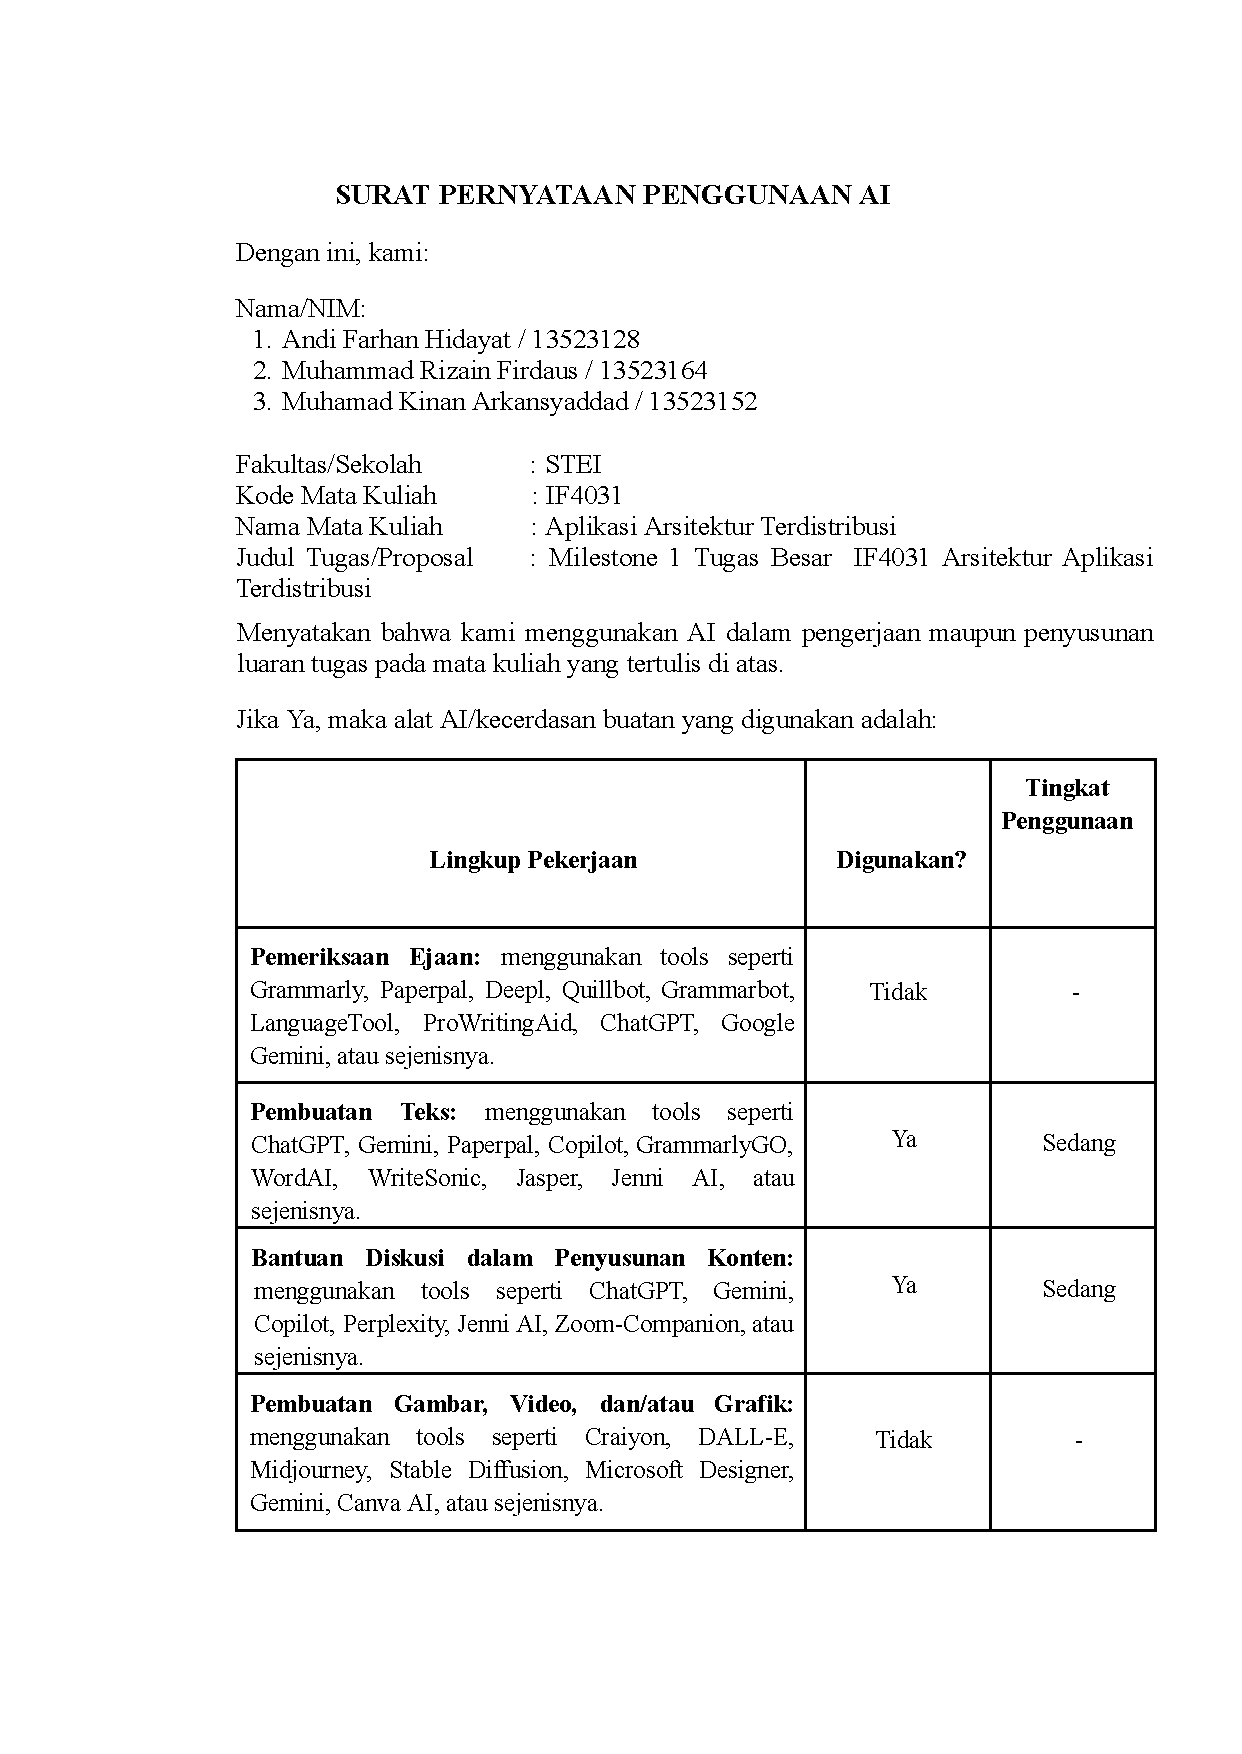
\includepdf[pages=-,pagecommand={\thispagestyle{empty}}]{IF4031_Surat-Pernyataan-AI_OrangSuksesAamiin.pdf}
